\subsection{Waves and Velocity} 

(Answers to M\Alph{subsection} problems are on page \pageref{waves_and_velocity_prob_answers}.)

\begin{Exercise}
If you haven't done so already, please read the following documents on Blackboard under ``Course Information:''
\begin{itemize}[nosep]
\item The Syllabus
\item ``On Working Together Honestly''
\item Homework Guidelines
\end{itemize}
(a)~If you could change any aspect of these course policies (or anything else about the course, I guess), what would you change?  You must make at least one suggestion for a change; no fair just answering that you're fine with whatever's currently there.  (b)~How serious are you about this request?  (Are you just suggesting a change because it was required, or because you genuinely think it would improve the course?)
\end{Exercise}

\begin{Exercise}[difficulty=1]
Use Appendix A in the lab manual to help you answer these dad jokes.  (a)~What do you call one millionth of a phone?  (b)~What do you call $2 \times 10^3$ mockingbirds? (c)~What do you call $1 \times 10^{-12}$ of a ``boo''?  (d)~What do you call one billionth of one billionth of a miser?  (e)~What do you call $10^{-6}$ meter? (this one's not actually a dad joke, but a serious question.) (f)~What space vessel held the dubious distinction of completing the Kessel Run in ``under 12 parsecs''?
\end{Exercise}

\begin{minipage}{0.74 \textwidth}
\begin{Exercise}[difficulty=1]
The right triangle shown in the figure has sides of length $A$, $B$, and $C$, and one of the angles is $\theta$.  (a)~Write an expression for $A$ in terms of $C$ and $\theta$.  (b)~Write an expression for $B$ in terms of $C$ and $\theta$.  
\answerspace{0.2in}
\end{Exercise}
\end{minipage}
\begin{minipage}{0.25 \textwidth}
\hspace{\fill}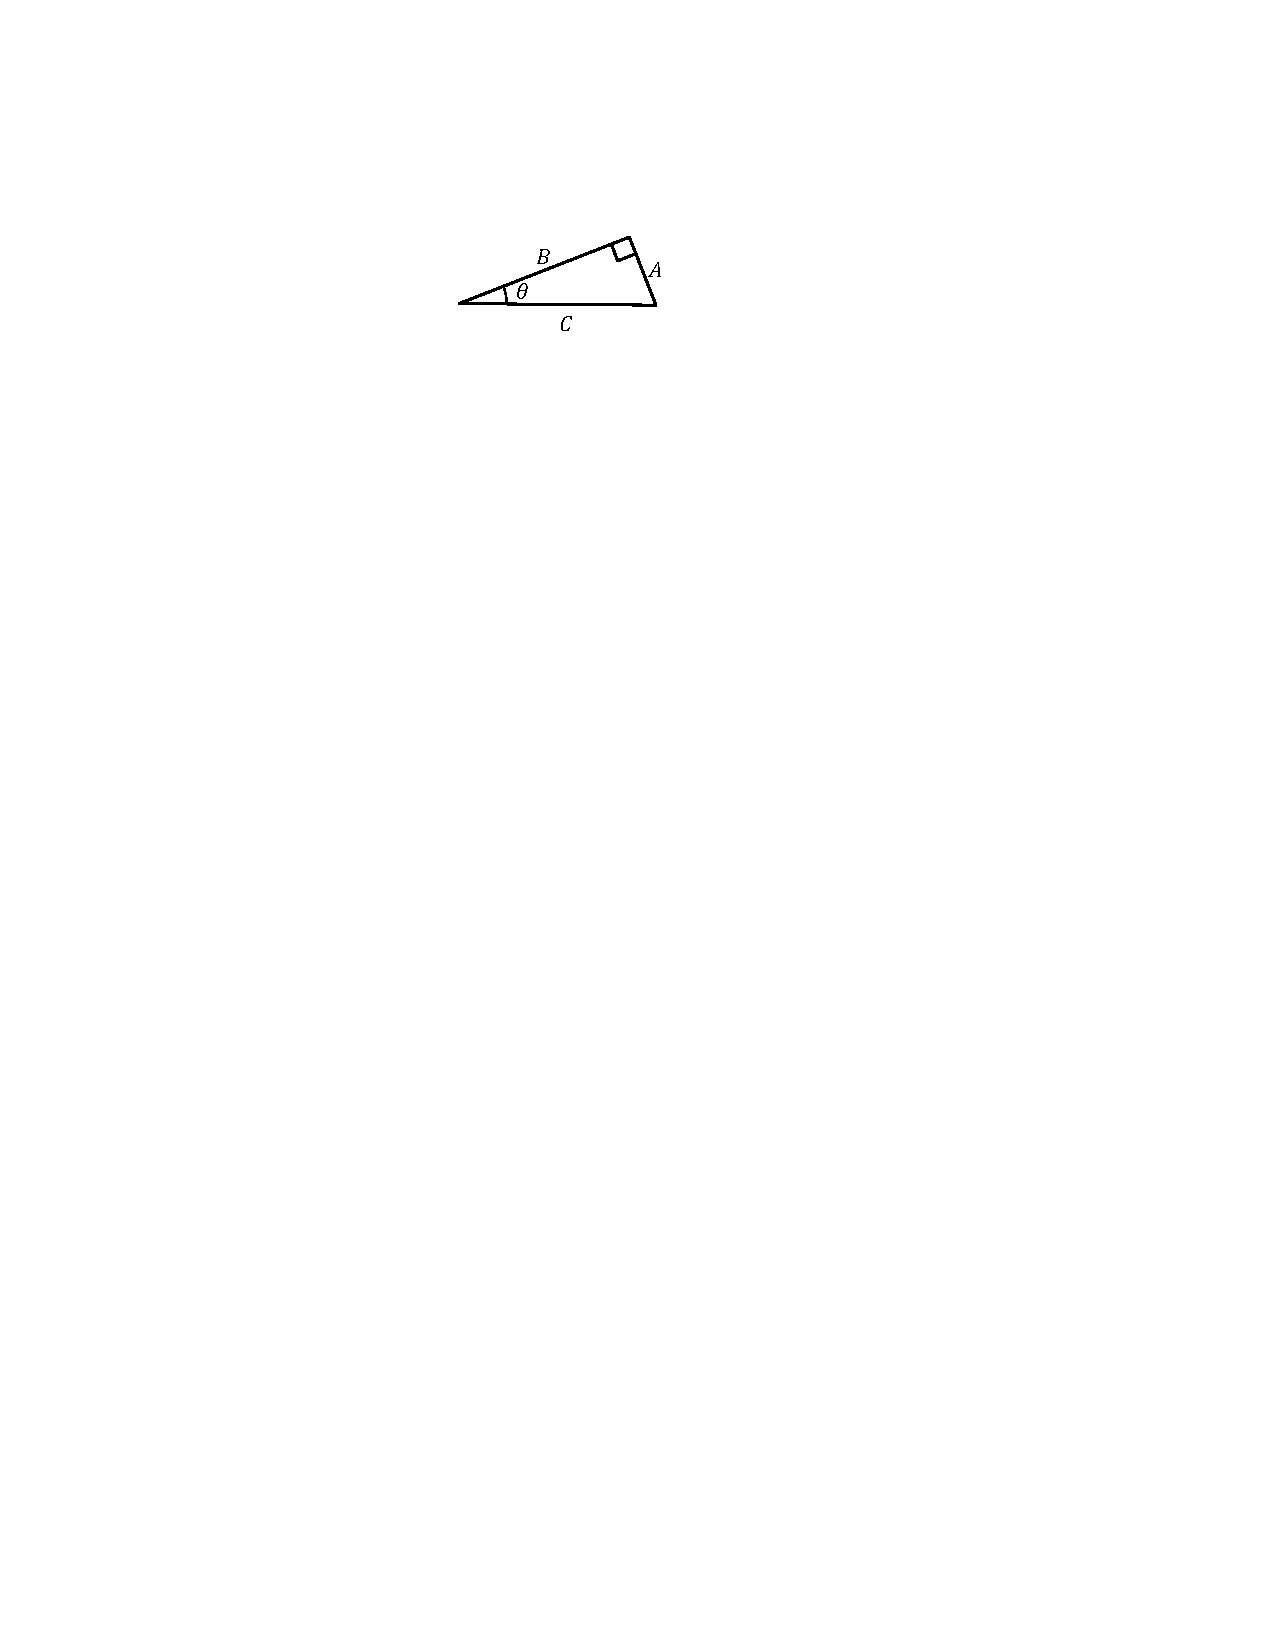
\includegraphics{M_problems/waves_velocity/triangle.pdf}
\end{minipage}
\begin{Answer}
(b) $B=C \cos\theta$
\end{Answer}

\begin{Exercise}[difficulty=1]
How long does it take for light to travel the distance of $L=80$~cm between the pair of slits and the detector in the experiment we did?  (The speed of light $c$ is $3 \times 10^8$~m/s, a value you will need to know for the rest of this course.)
\end{Exercise}
\begin{Answer}
2.67 ns
\end{Answer}

\begin{Exercise}
The nearest star to us is Proxima Centauri, which is 4.2465 light-years away from us.  If we could send a probe to that star at a constant speed one tenth of the speed of light ($v=0.1c$), how long would it take the probe to go there, snap one picture, and then return to Earth?
\end{Exercise}
\begin{Answer}
84.93 years
\end{Answer}

\begin{Exercise}
Imagine you are doing an experiment as in Lab~\ref{interference_lab}, shining light through two slits and observing the series of bright and dark spots created on a distant screen.
\begin{enumerate}[nosep,label=(\alph*)]
\item Suppose you increase the wavelength $\lambda$ of the light that you are using.  Does that make the bright spots on the screen \textit{closer together}, \textit{further apart}, or \textit{no change}?  
\item Now suppose that you keep the wavelength $\lambda$ of the light the same, but instead you increase the spacing $d$ between the two slits.  Does that make the bright spots on the screen \textit{closer together}, \textit{further apart}, or \textit{no change}?  
\item Finally, suppose you keep both $\lambda$ and $d$ the same, but instead you increase the distance $L$ from the slits to the screen.  (Say you increase it from 80~cm to 100~cm, for instance.)  Does that make the bright spots on the screen \textit{closer together}, \textit{further apart}, or \textit{no change}?  
\end{enumerate}
For parts (a) and (b) of this problem, it's worth thinking about each part for a few minutes with a pencil and paper, but then you should definitely check your answers using the little Mathematica applet interference.cdf that you used in class, which is available on Blackboard under ``Labs''.
\end{Exercise}
\begin{Answer}
(c) Increasing $L$ will increase the distance between bright spots on the screen.
\end{Answer}

\begin{Exercise}
Green laser light with a wavelength of $\lambda = 500$~nm is incident on two slits, separated by a distance $d=125~\mu$m, projecting a series of light and dark spots onto a distant screen, just as you did in Lab~\ref{interference_lab}.  Suppose that at one specific place on the screen, slightly to the left of the center, the distance from that spot on the screen to one of the two slits is exactly $1.75~\mu$m greater than the distance to the other slit.  (That is, the path difference $\Delta r$, in the diagram in Activity 3 of your lab, is exactly $\Delta r=1.75~\mu$m.)  Is that specific place on the screen a bright spot, or a dark spot?
\end{Exercise}
\begin{Answer}
It's a dark spot.  Of course, on your homework paper, you need to show your work and explain \textit{why} it's a dark spot.  Oh, by the way: yes, this problem does include an extraneous piece of information that you didn't need---you're welcome!  :-)
\end{Answer}


\begin{Exercise}
Laser light is incident on a pair of slits separated by a distance of $90~\mu$m.  When a screen is placed 1.4~meters behind the slits, bright spots on the screen are observed to be separated from each other by a distance of 8.3~mm.  What is the apparent wavelength of the laser light?
\end{Exercise}
\begin{Answer}
534~nm
\end{Answer}

\begin{Exercise}
Laser light with wavelength $\lambda=655$~nm is incident on a set of three narrow slits.  The outer slits are exactly $150~\mu$m apart, and a third slit lies exactly midway between them.  (a)~Consider only a set of rays directed at an angle
$\theta=0.25^\circ$ from horizontal.  When these rays eventually reach a screen (or a detector), will they combine in such a way that they produce an interference maximum, an interference minimum, or something in between?  (b)~If a screen is placed 1.25~meters away from these slits, at what locations $\Delta x$ relative to the centerline will the first three intensity maxima be found?
\begin{center}
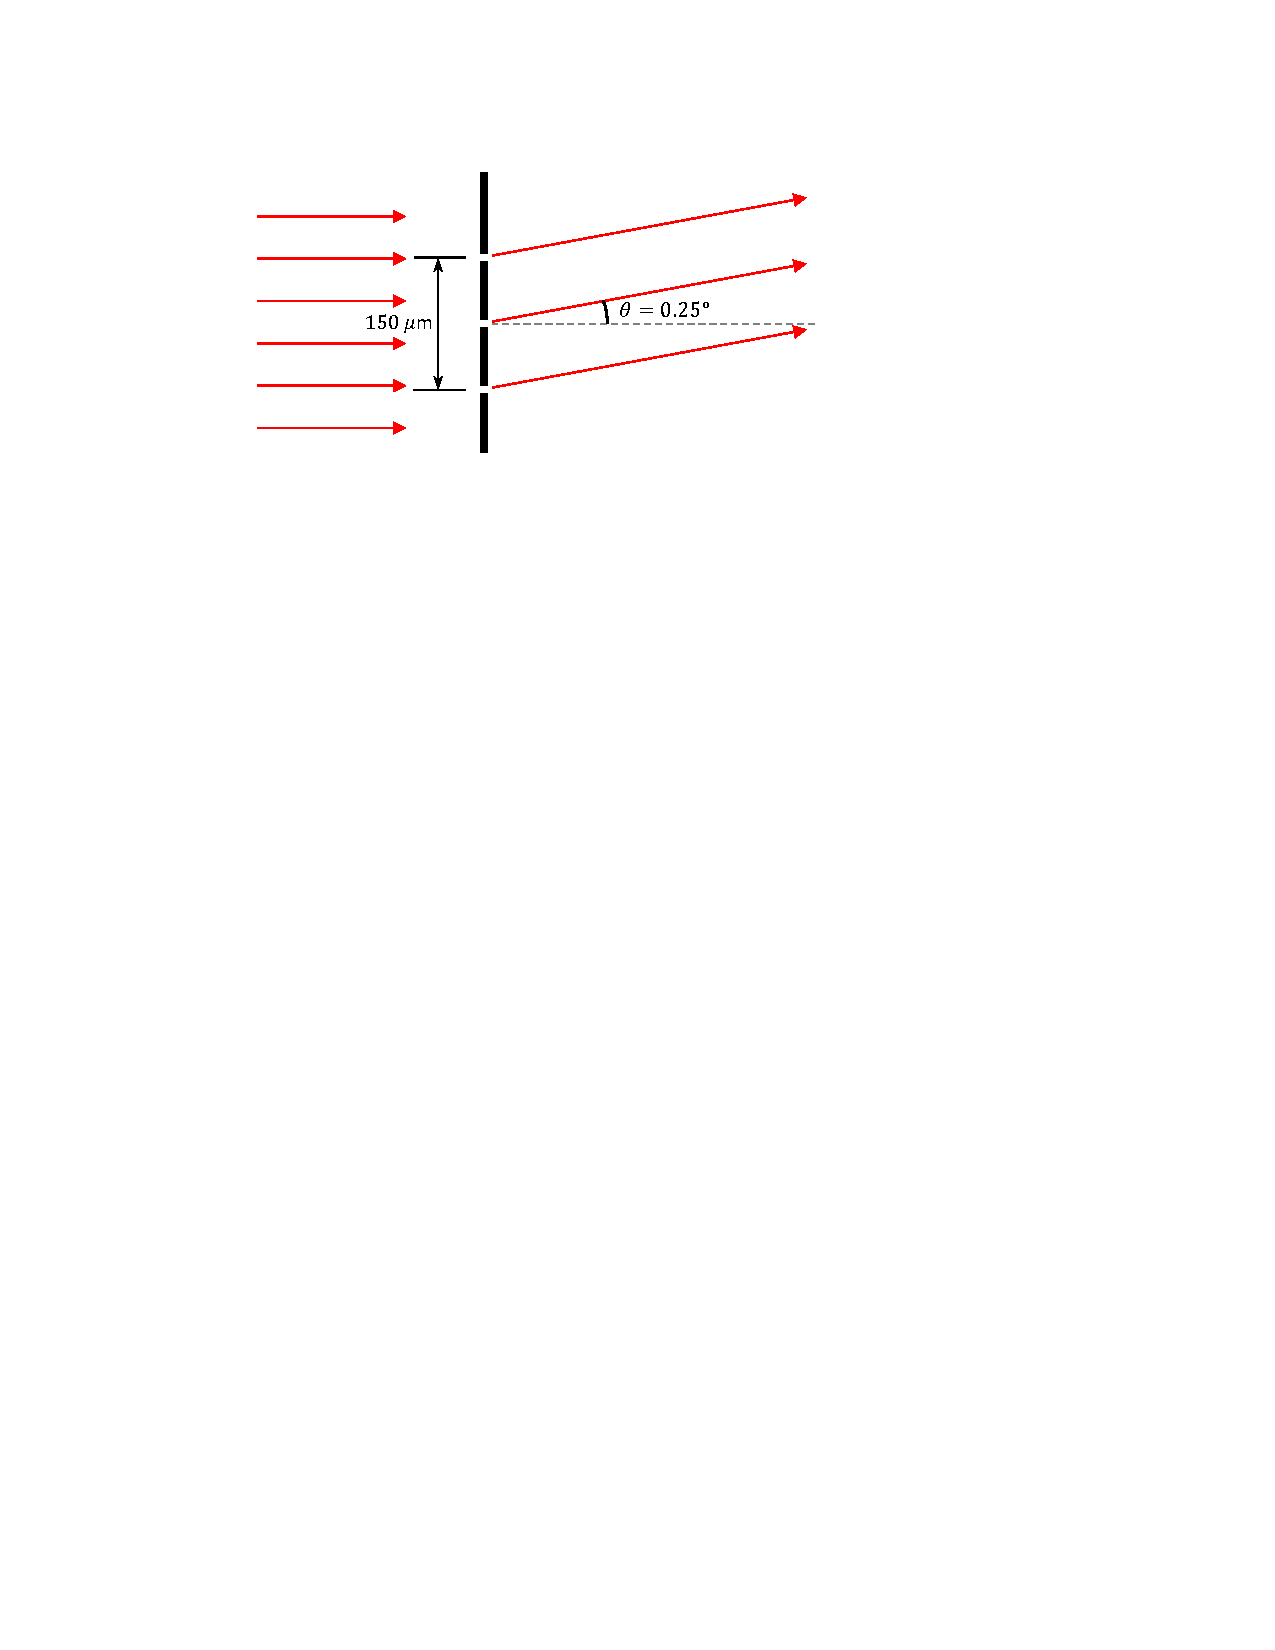
\includegraphics[scale=0.9]{M_problems/waves_velocity/three_slits.pdf}
\index{color page}
\end{center}
\end{Exercise}
\begin{Answer}
(a) Something in between.  (b) $\Delta x=0$~mm, $\pm 10.9$ mm, and $\pm 21.8$ mm.
\end{Answer}


\begin{Exercise}
Use the little Mathematica applet \filename{interference.cdf} that we've used in class to answer this question.  Start with two slits, and then increase the number of slits from 2 up to 3, 4, and 5.  (a)~As you increase the number of slits, what happens to the locations of the bright spots on the distant screen?  (b)~As you increase the number of slits, what happens to the intensity, or maximum brightness, of each bright spot?  (c)~As you increase the number of slits, what happens to the width of each bright spot?  (d)~Is a location on the screen that is an exact brightness minimum for two slits also always an exact brightness minimum for 3, 4, or 5 slits? \label{problem_number_of_slits}
\end{Exercise}

\begin{Exercise}
A ``diffraction grating'' is what you call a device with hundreds or thousands of slits for light to pass through, as opposed to just two or three or a dozen slits.  As you saw in problem \ref{problem_number_of_slits}, when you add more slits, the locations of the brightness maxima and minima do not change; you still have constructive interference at any angles for which 
$d \sin \theta = m\lambda$,
where $m$ is any integer.  
Suppose you shine red laser light with a wavelength of 625~nm on a diffraction grating with many slits, all spaced $3.5~\mu$m apart.
Calculate all of the angles $\theta$ at which constructive interference (bright spots) will be observed.
\end{Exercise}
\begin{Answer}
$0^\circ$, $10.3^\circ$, $20.9^\circ$, $32.4^\circ$, $45.6^\circ$, and $63.2^\circ$
\end{Answer}

\begin{Exercise}[difficulty=1]
Draw a quantitative position vs. time graph for the following motion, as you walk back and forth along an $x$ axis: 
\begin{itemize}[nosep]
\item You start at a position $x=+2$ m at time $t=0$.
\item First, you walk in the negative $x$ direction at a velocity $v=-2$ m/sec for 3 seconds.
\item Then you stop for 3 seconds.
\item Finally, you walk in the positive $x$ direction at velocity $v=+1$ m/sec for 3 seconds.
\end{itemize}
Note that ``quantitative'' means that your axes should have numbers, so a person looking at your graph could read a specific numerical value of your position at any given time from your graph.
\end{Exercise}


\begin{Exercise}
A cat is chasing a mouse across a large, 10-meter-wide room.  The cat starts at one end of the room, $x=0$, and runs at top speed ($v=6$~m/s) towards the mouse, who is at the center of the room, $x=5$~m.  At the same time, the mouse runs at $v=4$~m/s away from the cat, towards a mouse hole at the far end of the room, $x=10$~m.  (a)~Draw a single position vs. time graph with two lines on it, one representing $x$ vs. $t$ for the cat, and one representing $x$ vs. $t$ for the mouse.  (b)~Perhaps you remember from previous math classes that the general equation for a line is $y=mx+b$, or, in this case, $x=vt+x_0$, where $x_0$ represents the position at time $t=0$. Write an equation describing the position of the cat as a function of time, $x_{\rm cat}(t)$, using the numbers in this problem.  (c)~Write another equation for the position of the mouse as a function of time, $x_{\rm mouse}(t)$.  (d)~Does the mouse get away?
\end{Exercise}
\begin{Answer}
(b) $x_{\rm cat} =(6~{\rm m/s})t+0$ m  (d)~Hint: if the mouse does NOT get away, that would mean that there's some time $t$ when $x_{\rm cat} =x_{\rm mouse}$  that occurs BEFORE the mouse gets to the hole, right? 
\end{Answer}

\begin{Exercise}
From the pages from Griffiths' book Electrodynamics that are posted under ``Notes,'' give three examples of equations that are integrated into sentences or introduced differently from anything you did in your first writing assignment. For each example, write the sentence and say something intelligent about how the equation (or a part of the equation) functions in the sentence.  (For instance, does the equation function as the main clause of the sentence?  Or as a subordinate clause?  Is one of the variables in the equation obviously identifiable as the subject or predicate nominative of the sentence? If you are unsure of these grammatical terms, you can focus instead on the ways in which variables are defined either before or after the sentence, for instance by using ``where,'' after the equation, or in an appositive before the equation, etc.) 
\end{Exercise}



\bigskip\bigskip\bigskip
\pagebreak[3]
\textbf{Answers to Selected {\thesubsection} Problems:}
\label{waves_and_velocity_prob_answers}
%\shipoutExercise
\shipoutAnswer

\cleardoublepage
